\documentclass[t]{beamer}
%\usepackage{multimedia}		% for movies, sounds, animations...
\usepackage[ngerman,german,english]{babel}		% new german
\usepackage[utf8]{inputenc}		% input...

\usepackage{tabularx}			% local, only for this doc.

\usepackage[tamsWZ, blockBG, tams,engl]{tamsBeamer}
%-----------------------------------------------------------------------------
%-- options		------------------------------------------------------
%			tams	|	- TAMS		publication
%			cinacs		- CINACS	publication
%			engl		- english strings	[german]
%			uniWZ	|	- uni		watermark
%			tamsWZ	|	- tams+uni	watermark
%			cinacsWZ	- cinacs+uni	watermark
%			secToc	|	- toc repetition at each section
%			secTocA		- -"-, all sections: show
%					  replacement for toc in short docs
%			subsecToc	- toc repetition at each subsection
%			secNum  	- (sub)-section numbering
%			fullstep	- always step through items
%			noFoot		- footline	off
%			noPage		- page numbers	off
%			noAuth		- author	off
%			conference	- footline with \foottitle{...}
%			blockBG	|	- block, example etc. background
%			blockRound	- -"-, rounded+shadow


% fonts definitions			--------------------------------------
% ----------------------------------------------------------------------------
% default: cmss, OT1 fontenc		good with UniHH font "The Sans"
%					-> don't change fonts!
%\usepackage{times}			% other fonts
%\usepackage[T1]{fontenc}		%

% document definitions			--------------------------------------
% ----------------------------------------------------------------------------
\title		% title		-- option: short
  {Multitouch Robot Control}
\subtitle[B.Sc. Thesis]			% subtitle	-- option: short
  {Bachelor Thesis}

\author[M.~Steuer]{Merlin Steuer}

%\author[AutorA, AutorB]		% author	-- option: short
% {A.~Autor\inst{1} \and B.~Autor\inst{2}}%		-- option: \inst{...}
% style option: [tams] predefines institute...
% or define \institute{...}
%					% \inst{...} for different institutions
%\institute[Universities A and B]	% institution	-- option: short
%{ \inst{1}%
%  University of A\\
%  Department of A
%  \and
%  \inst{2}%
%  University of B\\
%  Department of B}

\date[24-apr-2018]			% event/date	-- option: short
  {24.~April 2018}

%\subject{TAMS, LaTeX, Folien}		% subject	-- option for pdf

% detailed information to be embedded in PDF		------------------- --
%\hypersetup{%
%  pdftitle={TAMS-Folien mit 'beamer'},
%  pdfauthor={Andreas Mäder, Universität Hamburg,
%        MIN-Fakultät, Fachbereich Informatik, TAMS},
%  pdfsubject={Präsentationen mit pdflatex erstellen},
%  pdfkeywords={TAMS, LaTeX, Folien}}


\usepackage[backend=bibtex8,
style=numeric,
citestyle=numeric,
alldates=edtf,
maxbibnames=99]{biblatex}

\addbibresource{Bachelorarbeit.bib}  
\renewcommand*{\bibfont}{\footnotesize}

% document starts here			--------------------------------------
% ----------------------------------------------------------------------------
\begin{document}

% titlepage				--------------------------------------
%\frame[plain]{\titlepage}		% suppress head- and footlines
\frame{\titlepage}

% toc					--------------------------------------
\begin{frame}[allowframebreaks]
  \frametitle{\tocName}
  \tableofcontents
  %\tableofcontents[pausesections]	% step through sections
\end{frame}

\section{Introduction}

\begin{frame}{Merlin Steuer}
\begin{itemize}
	\item Part-time student
	\item B.Sc. Informatik since WiSe13
	\item 2steuer@informatik.uni-hamburg.de
	\item Questions? Make some noise!
\end{itemize}
\end{frame}

\subsection{Motivation \& Objective}

\begin{frame}{Motivation \& Objective}
\begin{itemize}
	\item Robots get more and more ubiquitous
	\item Robots enter domestic space\cite{Forlizzi2006}
	\item Interfaces have to be easy and intuitive
\end{itemize}

$\Rightarrow$ A simple, intuitive remote control interface to complex robots shall be developed.

\begin{itemize}
	\item Multitouch gestures well known
	\item Android tablet computer
\end{itemize}
\end{frame}

\begin{frame}{Grasp Synergies}
\begin{itemize}
	\item Research at the TAMS group \cite{Bernardino2013}
	\item PCA on human grasp postures
	\item Eigenvectors in matrix $S$ (called \textit{Synergy} here)
	\item Offset $s_0$~$=$~mean joint values 
\end{itemize}

\begin{equation}
\theta = s_0 + S\alpha
\end{equation}

\begin{itemize}
	\item $\alpha \in \mathbb{R}^{21}$\quad input amplitudes
	\item $\theta \in \mathbb{R}^{21}$\quad joint angles of the hand
\end{itemize}

$\Rightarrow$ Map properties of gestures to $\alpha$

\end{frame}

\begin{frame}{Grasp Synergies}
\begin{figure}
	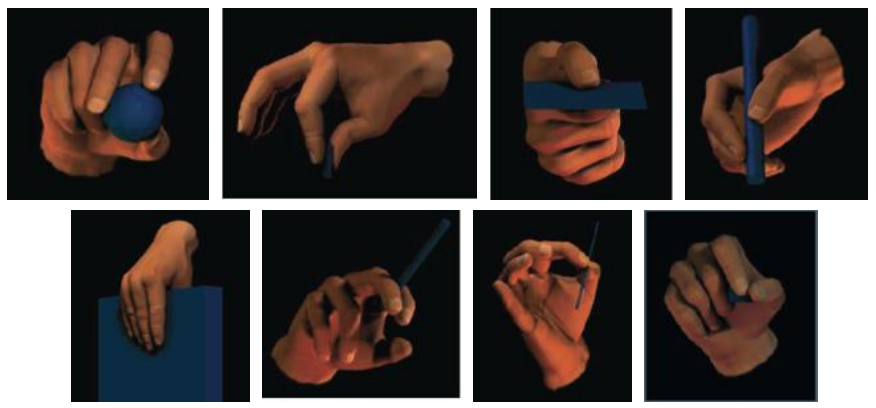
\includegraphics[height=0.6\textheight]{assets/pres/grasps.PNG}
	\caption{Grasp synergies recorded by \citeauthor{Bernardino2013}\cite{Bernardino2013}}
\end{figure}
\end{frame}

\begin{frame}{Direct Fingertip Mapping}
\begin{itemize}
	\item Research done by \citeauthor{conf:humanoids:TohHLBZP12} \cite{conf:humanoids:TohHLBZP12}
	\item Grasp actions $\rightarrow$ fingertip movements in a plane
\end{itemize}

$\Rightarrow$ Map fingertips on touch screen to a plane in $3D$ space
\end{frame}

\begin{frame}{Direct Fingertip Mapping}
\begin{figure}
	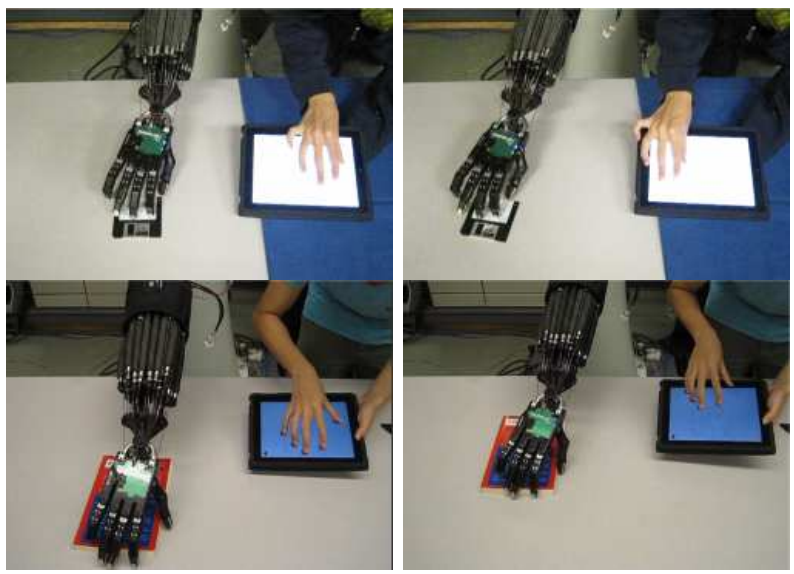
\includegraphics[height=0.6\textheight]{assets/pres/dftm_toh.PNG}
	\caption{Examples from \citeauthor{conf:humanoids:TohHLBZP12}\cite{conf:humanoids:TohHLBZP12}}
\end{figure}
\end{frame}

\subsection{Related Work}
\subsection{Hardware}
\subsection{ROS}
\subsection{Inverse Kinematics}

\section{User Interface}
\section{Implementation}
\subsection{Software Architecture}
\subsection{Synergy Approach}
\subsection{Direct Fingertip Mapping}

\section{Evaluation \& Outlook}

\section{Bibliography}

\begin{frame}[allowframebreaks]{Bibliography}
\printbibliography
\end{frame}

\section*{I'm done.}

\begin{frame}[c]
\centering
Thank you.
\end{frame}

\end{document}
